\renewcommand{\leftmark}{NOMINATION DES TECHNOLOGIES}


\chapter{Rappels et nomination des technologies}\label{chap1}

\section{Signal radio}

Un signal est une variation dans l'espace ou dans le temps d'une quantité physique contenant de l'information. Un signal peut être continu ou discret, on le nomme alors respectivement analogique ou numérique. Le type de signal dépend notamment de l'information qu'il contient. Un signal analogique est continue en amplitude, ce qui veut dire qu'il peut contenir un nombre infini de valeur, ainsi que prendre toutes les valeurs possibles, là où un signal numérique contient généralement un nombre fini de valeur (par exemple des 0 et 1).
Les deux catégories ne sont pas incompatible car il est souvent nécessaire en télécommication de pouvoir passer de l'un à l'autre.

\vspace{0.1cm}

L'utilisation de signaux radio en télécomunication confère de nombreux avantages, comme la portée, la vitesse de transmission  ou encore le coût de propagation. Pouvoir transporter de l'information sans avoir recours à du support matériel complet (pas besoin de cable, le signal passe dans l'air) réduit\\ considérablement le cout de la transmission. Ajouté à cela, il est possible d'adapter un signal pour le rendre compatible avec diverse canaux de transmission et de réception, grâce à la modulation. La modulation est une technique permettant de modifier les propriétés du signal lui permettant de transporter de l'information.

\newpage

En télécommunication, les signaux sont des ondes électromagnétiques appelées signal radio. Les signaux comportent de nombreuses caractéristiques qui les déterminent: 

\vspace{0.1cm}



la fréquence, mesurée en Hertz ($Hz$). Elle détermine le nombre de cycle qu'accomplit le signal par seconde. Une onde radio possède une fréquence entre 9kHz et 300GHz.

\vspace{0.1cm}

La largeur de spectre, elle dépent de la fréquence car c'est l'écart entre la plus haute et la plus basse fréquence du signal. Une plus grande largeur permet de transmettre plus d'informations, mais consomme plus d'énergie.

\vspace{0.1cm}

L'amplitude. Selon le type de signal l'attribut possède différentes fonctions. Dans le cas d'un signal analogique l'amplitude détermine la magnitude de l'onde pour n'importe quel point dans le temps. Dans un signal numérique l'amplitude est interprétée différemment. Les signaux numériques sont encodés avec des valeurs discrètes, où chaque valeurs repésente un niveau (par exemple 0 ou 1). L'amplitude permet de faire la disctinction entre ses niveaux.

\vspace{0.1cm}

la puissance, mesurée en Watt (W). C'est la force du signal, un attribut important pour la réception du signal notamment. Bien que le Watt soit utilisé pour décrire la puissance à l'émission ou la réception, les variations de puissances sont généralement exprimées en décibels (dB). Le décibel est une unité logarithmique permettant de mesurer plus facilement les realtions entre les différents niveaux de puissance.

\vspace{0.1cm}

le \textit{Signal to Noise Ratio} (SNR). Cet attribut mesure la qualité du signal. une valeur élevée indique que le pourcentage de bruit est faible.

\vspace{0.1cm}

le \textit{Bit rate}, ou le taux de transmission mesure la quantité de donnée transmise en bit par seconde. Cet attribut est exclusif aux signaux numériques. On parle de \textit{Baud rate} pour mesurer la quantité de symboles transmise par seconde. Ce n'est pas excatement l'équivalent du bit rate car un symbole peut contenit plusieurs bits, mais le Baud rate est utilisé pour les signaux numériques et analogiques.



\section{Traitement du signal}

\subsection{Modulation}

La réception d'un signal radio nécessite une antenne dont les dimensions dépendent de la longueur d'onde du signal. La longueur d'onde d'un signal représente la distance entre deux points consécutifs de même phase dans l'onde. La longueur d'onde s'obtient par la formule suivante :

\begin{equation}\label{eq1}
c = f * \lambda
\end{equation}

où $c$ est la vitesse de la lumière,

$f$ est la fréquence,

$\lambda$ est la longueur d'onde.

\vspace{0.1cm}

Il est donc possible d'adapter les charactéristiques d'un signal pour le rendre compatible à différentes antennes, via la modulation. La modulation est le procédé par lequel un ou plusieurs attributs du \textit{baseband signal} (le signal modulant, contenant l'information à transmettre) vont être altéré par le \textit{carrier signal} (un signal porteur, utilisé pour être combiné avec le signal modulant) pour devenir un signal modulé, le \textit{modulated signal}.

En plus de sa compatiblité, un signal modulé a l'avantage d'être facilement transmissible sur une grand portée sans perdre en puissance.

\vspace{0.1cm}

Parmis ces différents attributs, certains sont utilisés pour effectuer une modulation. Les trois modulations les plus utilisés sont basées sur les attributs de la fréquence, l'amplitude et la phase. La modulation en fréquence (\textit{Frequency modulation, FM}) consiste à encoder l'information en faisant varier la fréquence en maitenant l'amplitude constante. La modulation en amplitude (\textit{Amplitude modulation,AM}) est le procédé inverse, c'est à dire encoder l'information en faisant varier l'amplitude tout en gardant la fréquence constante. La modulation en phase (\textit{Phase Modulation, PM)} fait varier la phase de la porteuse proportionellement à l'amplitude instantannée du baseband signal.

\vspace{0.1cm}

La modulation en amplitude est plus ancienne et est encore utilisée dans beaucoup de systèmes. Cette technique possède moins de contrainte et est notamment plus simple à implémenter.

\vspace{0.1cm}

Soient $u(t)$ un baseband signal et $v(t)$ un carrier signal, la modulation en amplitude s'effectue en multipliant les deux signaux pour obtenir le signal modulé 

\begin{equation}\label{eq2}
s(t) = u(t) . v(t)
\end{equation}

Prenons par exemple 

$u(t)$ = $sin(2\pi f_{u}t)$ avec $f_{u}t$ = 5 Hz,

$v(t)$ = $cos(2\pi f_{c}t)$ où $f_{c}t$ = 50 Hz.

La Figure \ref{term1} montre le signal modulé $s(t)$ via la modulation en amplitude.

\newpage

\begin{figure}[h]
\centering

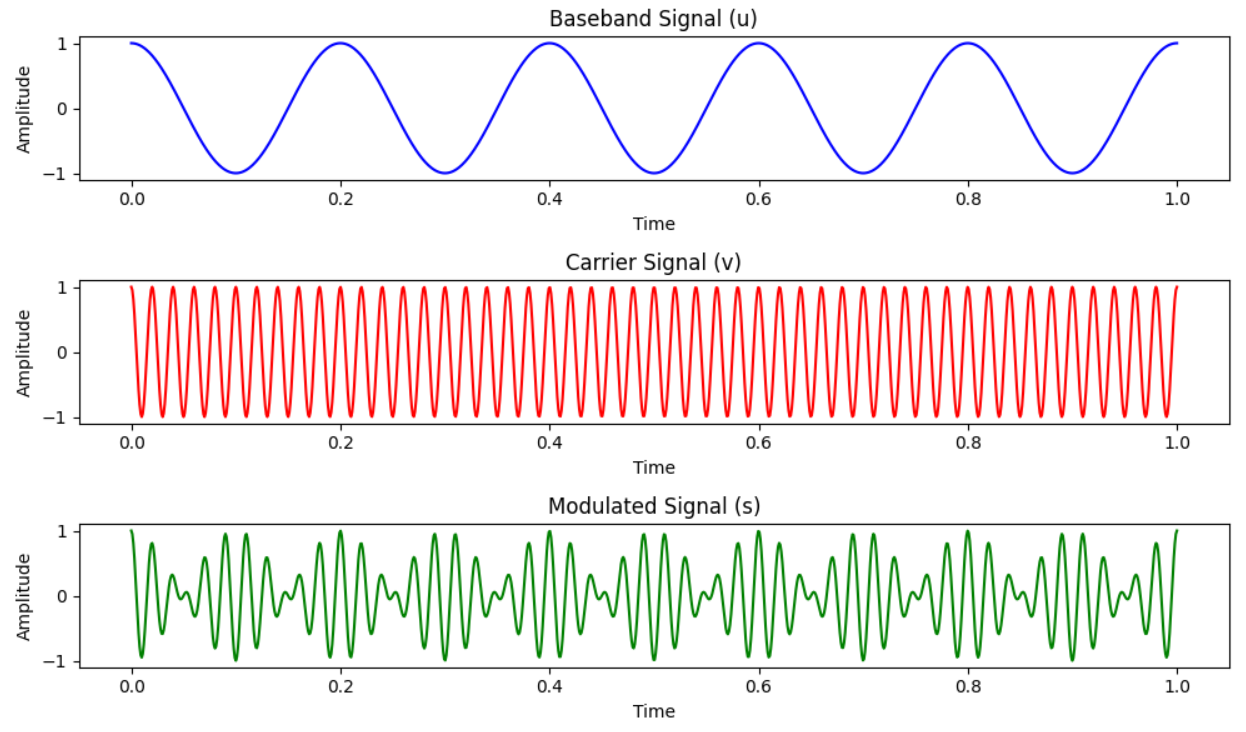
\includegraphics[scale=0.5]{images/AM_mod.PNG}
\caption{Exemple de modulation en amplitude}\label{term1}
\end{figure}


La modulation en fréquence permet d'obtenir des transmissions de meilleures qualités plus résistantes à leur environement tout en gardent une puissance d'émission constante. 

\vspace{0.1cm}

Soient $u(t)$ un baseband signal et $v(t)$ un carrier signal, le signal modulé en fréquence $s_{fm}(t)$ est le résultat suivant :

\begin{align}
    u(t) &= \sin(2\pi f_{u}t) \\
    v(t) &= \cos(2\pi f_{c}t + \phi_{c}) \\
    s_{fm}(t) &= \cos\left(2\pi f_{c}t + \Delta f \cdot u(t) \cdot t + \phi_{c}\right)
\end{align}

\vspace{0.1cm}

Prenons par exemple

\vspace{0.1cm}

$u(t)$ = $sin(2\pi f_{u}t)$ avec $f_{u}t$ = 5 Hz,

$v(t)$ = $cos(2\pi f_{c}t + \phi_{c})$ où $f_{c}t$ = 50 Hz.

\vspace{0.1cm}

La Figure \ref{term2} montre le signal modulé $s_{fm}(t)$ via la modulation en fréquence pour une phase initale ddu carrier signal $\phi_{c}$ = 0 avec une dérivation en fréquence $\Delta f$ = 10Hz.

\newpage

\begin{figure}[h]
\centering

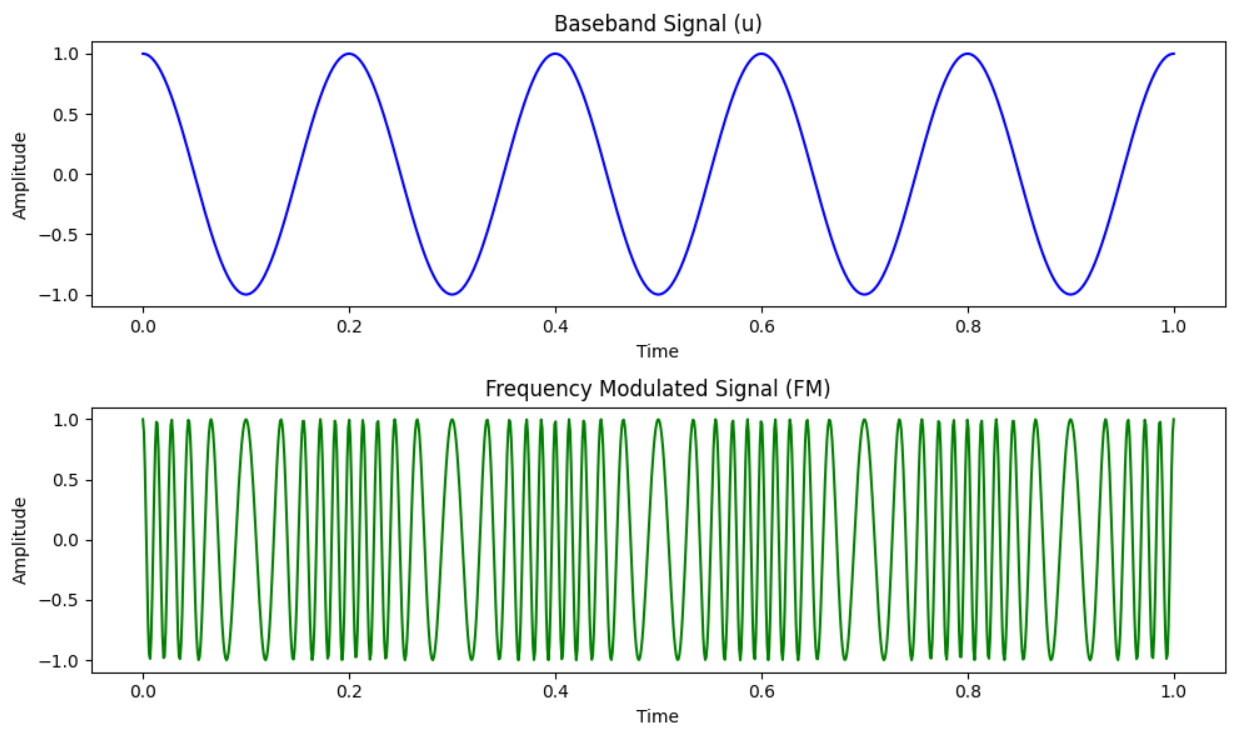
\includegraphics[scale=0.5]{images/FM_mod.PNG}
\caption{Exemple de modulation en fréquence}\label{term2}
\end{figure}

La modulation en phase permet généralement d'obtenir une meilleur utilisation de la bande passante que les autres modulations car les variations de phase peut encoder plus d'informations, ce qui augmente la quantité de données transmises.

Soient $u(t)$ un baseband signal et $v(t)$ un carrier signal, le signal modulé en phase $s_{pm}(t)$ est le résultat suivant :

\begin{align}
    u(t) &= \sin(2\pi f_{u}t) \\
    v(t) &= \cos(2\pi f_{c}t + \phi_{c}) \\
    s_{pm}(t) &= \cos\left(2\pi f_{c}t + K_{p} \cdot u(t)\right)
\end{align}

\vspace{0.1cm}

Prenons par exemple

\vspace{0.1cm}

$u(t)$ = $sin(2\pi f_{u}t)$ avec $f_{u}t$ = 5 Hz,

$v(t)$ = $cos(2\pi f_{c}t + \phi_{c})$ où $f_{c}t$ = 50 Hz.

\vspace{0.1cm}

La Figure \ref{term3} montre le signal modulé $s_{pm}(t)$ en phase pour une phase initale ddu carrier signal $\phi_{c}$ = 0 avec un index de modulation de phase $K_{p}$ = 8.

\newpage

\begin{figure}[h]
\centering

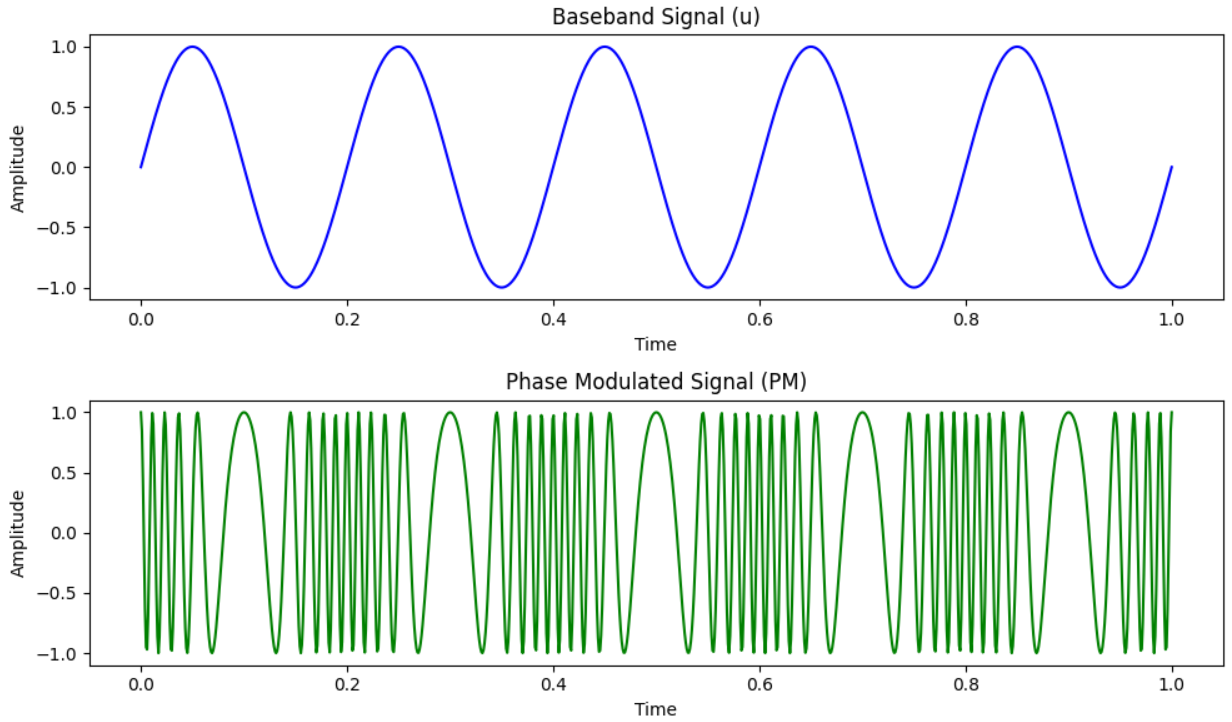
\includegraphics[scale=0.5]{images/PM_mod.PNG}
\caption{Exemple de modulation en phase}\label{term3}
\end{figure}

\subsection{Gestion du bruit}

L'un des attributs cités concerne le bruit. Un signal est toujours affecté de petites fluctuations plus ou moins importantes, et dont les origines peuvent être diverses. Ces perturbations, appelée bruit ou \textit{noise} en télécommunication se définissent par l'altération non souhaitée de l'intégrité d'un signal. Le bruit peut prendre différentes formes, des perturbations essentiellement impulsionnelles engendrées par des commutations de courants ou alors du bruit de fond généré dans les câbles et les composants électroniques en raison
des mécanismes statistiques de la conduction électrique. Il est possible de réduire voir éliminer l'influence des perturbations impulsionelles. En revanche, le bruit de fond est lui irreductible. Tout signal sans bruit n'existe pas, même à l'émission. Il est cependant possible que le bruit devienne invisible si son niveau est très faible. L'attribut SNR est donc un critère de la qualité du signal.


\subsection{Transformée de Fourier}

Pour effectuer une analyse de signal, sa représentation est capitale. Les Figure 1 et 2 représentent des signaux en fonction du temps écoulé. Il est possible de représenter des signaux selon une autre composante, la fréquence.

\vspace{0.1cm}

La transformée de Fourier est un outil fondamental utilisé pour analyser et décomposer des signaux complexes en composantes fréquentielles. En transformant un signal dans le domaine temporel en sa représentation dans le domaine fréquentiel, la transformée de Fourier révèle les différentes composantes fréquentielles présentes dans le signal. En fonction du type de signal, la transformée de Fourier est adaptée.

\vspace{0.1cm}

Pour les signaux continus, la \textit{CFT} (Transformée de Fourier continue) convertit une fonction du temps en fonction de la fréquence en intégrant le signal par rapport aux sinusoïdes de toutes les fréquences possibles. Cette transformation fournit les informations d'amplitude et de phase pour chaque composante de fréquence présente dans le signal.

\vspace{0.1cm}

Pour les signaux discrets et échantillonnés, la \textit{DFT} (Transformée de Fourier discrète) calcule un ensemble fini de composantes de fréquence. Il est calculé à l’aide d’un nombre fini d’échantillons, ce qui donne des composantes de fréquence discrètes. Il existe un méthode simplifiée pour les signaux discrets appelé \textit{FFT (Fast Fourier Transform)}\cite{fft}. Il s'agit d'un moyen plus rapide de calculer la transformée de Fourier, en particulier pour les signaux numériques comportant un grand nombre de points de données. L'avantage principal de cet algorithme permet de réduire le temps de calcul en divisant la DFT en sous problèmes. La FFT est une méthode très utilisée pour l'analyse de signaux.

\newpage

\section{LoRa}

\textit{LoRa} (Long Range) est une technologie de communication sans fil qui permet de transmettre des données sur de longues distances avec une faible consommation d'énergie. Elle a été développée par la société française Cycleo et est maintenant gérée par la fondation LoRa Alliance, qui regroupe plusieurs entreprises et organisations du monde entier.

\vspace{0.1cm}

LoRa est principalement utilisée dans l'IoT. Elle se distingue par sa portée étendue, qui peut atteindre plusieurs kilomètres en milieu urbain et plusieurs dizaines de kilomètres en milieu rural, ainsi que par sa faible consommation d'énergie, qui permet de prolonger la durée de vie des appareils connectés. Une longue portée avec un puissance limitée induit une plus faible bande passante que les autres technologies sans fil (le Wifi, la 4G, Bluetooth etc).

\vspace{0.1cm}

LoRa utilise une bande de fréquences qui varie selon les régions du monde où LoRa est déployée :

\vspace{0.1cm}

\begin{itemize}
\item en Europe, la bande de fréquences autorisée est comprise entre 863 et 870 MHz, ce qui correspond à l'\textit{ISM radio band}, un bande dédié aux recherches qui ne nécessite pas de license d'émission.
\item aux États-Unis, elle se situe entre 902 et 928 MHz,
\item en Chine, la fréquence autorisée varie entre 779 et 787 MHz,
\item les régions restantes ont elles aussi une fourchette unique.
\end{itemize}

\vspace{0.1cm}

La technologie LoRa utilise la modulation appelé \textit{Chirp Spread Spectrum Modulation} (CSS). La modulation CSS utilise un signal chirp, c'est à dire un signal modulé en fréquence linéaire. Ce signal a une amplitude constante mais balaie tout le spectre de la bande passante de manière linéaire dans une période de temps définie. Cette technique de modulation sera détaillée à la section \ref{css}

\vspace{0.1cm}

La technologie LoRa utilise également une technique de multiplexage en temps partagé (\textit{Time Division Multiple Access}) pour permettre à plusieurs appareils de partager la même bande de fréquences de manière à maximiser l'utilisation de la capacité de transmission. Elle utilise également une technique de diffusion de données (\textit{multicast}) pour envoyer les mêmes données à plusieurs appareils simultanément, ce qui permet de réaliser des économies de bande passante et d'énergie (source : \href{https://resources.lora-alliance.org/technical-trainings/lorawan-device-to-device-multicast-communications}{LoRa Alliance})

\vspace{0.1cm}

En plus de sa portée étendue et de sa faible consommation d'énergie, LoRa se distingue par sa sécurité de transmission, qui est assurée grâce à l'utilisation de codes de sécurité uniques et à la possibilité de chiffrer les données transmises. Lora n'est pas exclusivement lié au protocole LoraWan. Ce protocol sera décrit en détails à la section \ref{lorawan}. Si LoRa opère à un niveau plus bas que la plupart des protocoles réseau, LoRaWan via son infrastructure (notament les \textit{gateway} permet entre autre aux appareils LoRa de pouvoir utiliser différents protocoles et d'être compatibles avec un grand nombre de protocoles de communications comme \textit{TCP/IP (transport layer protocol), HTTP (hypertext transfer protocol ou MQTT(message queuing telmetry transport)}.

\vspace{0.1cm}

Toutes ces  particularités font de LoRa une technologie complémentaire à celles déja existantes plutot que rivale.
LoRa se compose de deux éléments principaux : la couche physique de la technologie et LoRaWAN, la couche MAC (\textit{Media Access Control}, une sous couche de la couche liaison de données dans le modèle OSI \textit{Open Systems Interconnection}. la couche physique de LoRa gère la fréquence radio ainsi que la modulation. LoRaWAN gère les aspects réseaux comme la sécurité, la propagation, l'adressage et la sécurité.

\subsection{couche physique LoRa}

\subsubsection{Découpage de la couche physique}

\begin{figure}[h]
\centering

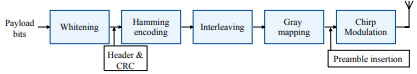
\includegraphics[scale=1]{images/physical_lora_rx.PNG}
\caption{Etapes de la transformation des données dans un émetteur LoRa\cite{loraphy}}\label{term4}
\end{figure}


Les étapes de la conception de l'envoi de données dans la couche physique de LoRa sont montrés dans la figure \ref{term4} :

\vspace{0.1cm}

\begin{itemize}
\item Le codage de canal (\textit{channel coding}) est une technique utilisée dans les systèmes de communication sans fil pour améliorer la robustesse et la fiabilité de la transmission des données. Dans le cas de LoRa, le codage de canal utilise le \textit{Forward Error Correction (FEC)} pour corriger les erreurs causées par du bruit. La méthode FEC ajoute de l'information redondante sur les données.
\item Le mélange de canal (\textit{channel interleaving}) suit le codage de canal.  
Cette technique consiste à réarranger les bits ou les symboles de données en les dispersant sur plusieurs canaux (ici on fait référence à des streams ou a des bandes de fréquences spécifiques plutôt qu'à des canaux physiques). Cela permet de réduire l'impact de \textit{burst errors}, des erreurs consécutives.
\item Le blanchiment de canal (\textit{channel withening)} est la dernière étape avant la modulation du signal.
Cette technique consiste à utiliser une transformation aléatoire ou pseudo-aléatoire des données avant de les transmettre, de manière à répartir le spectre des fréquences de la transmission sur une large gamme de fréquences. C'est une technique mathématique qui consiste a effectuer une transformation linéaire des données avec un matrice de covariance en un nouveau set de données dans la covariance est la matrice d'identitée. Le du blanchiment est de réduire la corrélation entre les différentes composante fréquencielles et assurer que le signal possède une puissance similaire tout le long de son spectre.
\item La modulation CSS est l'étape principale de LoRa. En effet, les étapes précédentes sont communes à de nombreuses technologies, mais la particularité de LoRa provient de la modulation. Cette étape est détaillée dans la section \ref{css}.
\end{itemize}

\vspace{0.1cm}

Chacune des étapes décrites doit être inversément réalisée pour le récepteur. Ainsi pour la récupération de donnée à l'arrivée, l'appareil récepteur gère la démodulation, le déblanchiment, le démellement et de décodage.

\vspace{0.1cm}

Cette analyse a été faite en \textit{Reverse Engeneering} par Alexandre Marquet, Nicolas Montavont et Georgios Z. Papadopoulos \cite{lorareverse}. Le reverse engineering consiste à analyser un produit ou un système afin de comprendre comment il fonctionne ou d'identifier ses principes de conception. Dans le contexte de LoRa, le reverse engineering examine la technologie derrière LoRa afin de comprendre ses principes de base et sa conception.


\subsubsection{Modulation CSS}\label{css}

Contrairement aux modulation classique en amplitude ou en fréquence, la modulation CSS étale le signal sur une large bande de fréquence. La modulation en fréquence est linéaire et utilise des chirps. un chirp est un signal dont la fréquence change en continue tout en conservant une amlitude constante. Il existe deux types de chirps : les $upchirp$ et $downchirp$.
Dans un upchirp la fréquence augmente avec le temps tandis que dans un downchirp la fréquence diminue. Soit $s_{chirp}(t)$ un signal chirp avec

\begin{equation}\label{eq3}
s_{chirp}(t) = sin(2\pi(f_0 + (\frac{f_1 - f_0}{T})t)t)
\end{equation}

alors la figure \ref{term5} montre $s_{chirp}$ en fonction du temps où $f_0$ = 10Hz, $f_1$ = 100Hz et $T$ = 1 seconde. On observe que le signal oscille de plus en vite plus vite au fur et à mesure que le temps augmente.

\begin{figure}[h]
\centering

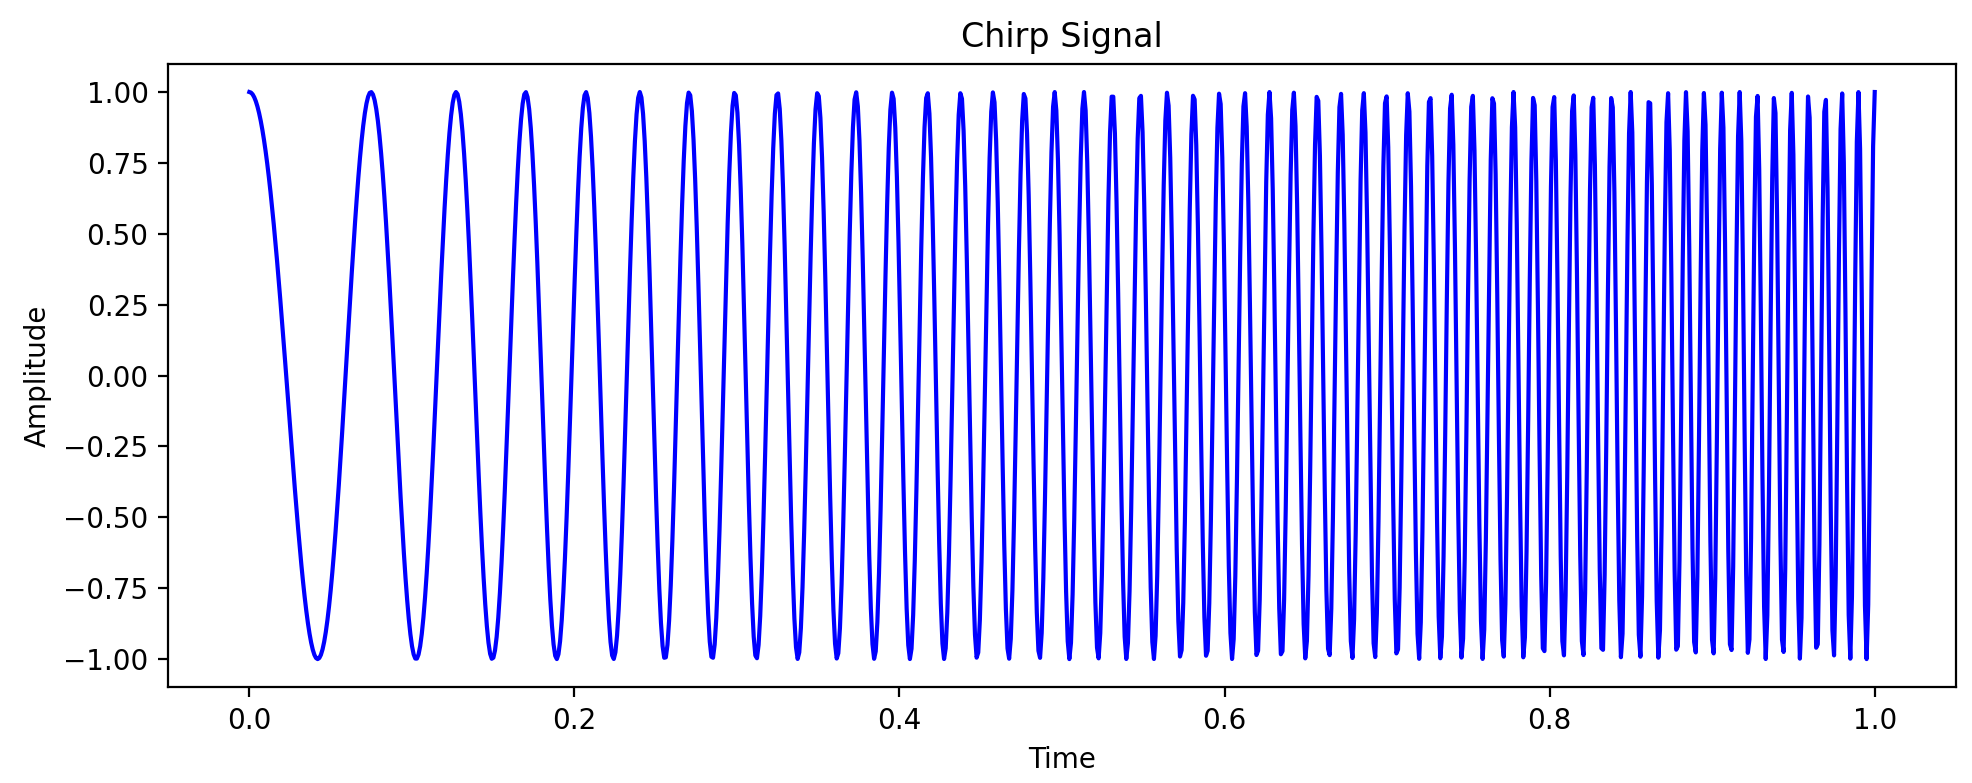
\includegraphics[scale=0.18]{images/CSSupchirp.png}
\caption{Example d'un signal modulé en upchirp en fonction du temps}\label{term5}
\end{figure}

\vspace{0.1cm}

Le signal est donc séparé sur une large bande de fréquence, permettant par exemple plusieurs transmissions sans causer d'interférence.
La modulation CSS est l'une des principales contributions au fait que LoRa possède une faible consommation et une longue portée. Cette technioque est très bien intégrée aux appareils a faible puissance utilisé par LoRa.

\subsubsection{Spreading factor}

LoRa permet d'envoyer des paquets sur une longue distance à faible puissance. Selon l'environement dans lequel les appareils LoRa sont présents, il peut être utile de pouvoir ajuster certaines capacités.

\vspace{0.1cm}

Le facteur d'étalement (\textit{Spreading Factor, SF}) permet de déterminer le taux de variation de fréquence pour un signal. Modifier le spreading factor ajuste différentes propriétés de la communications \cite{thethingsnetworkSF}. Par exemple, si on augmente le spreading factor, les quatre conséquences principales sont :

\vspace{0.1cm}

\begin{itemize}
\item l'augmentation de la portée. En effet augmenter le SF réduit le bitrate et augmente le \textit{processing gain} (l'augmentation de la puissance du signal atteint en l'étalant sur une plus large bande).
\item Augmentation de la résistance aux interférences. Comme le signal est étalé sur une bande plus largeur, il y a moins de risque de subit des interférences.
\item Plus petit débit de données. Le spreading factor controle le taux de chirp, et du coup la vitesse de transmission de donnée. Augmenter le speading factor signifie ralentir la vitesse d'émission des chirps. Pour chaque augmentation du spreading factor, le taux de transmission de donnée est réduit de moitié.
\item Plus faible consommation. Les données transmises à un taux plus faible consomment moins d'énergie, ce qui prolonge la durée de vie des appareils dont l'économie d'énergie est une priorité.
\end{itemize}

Diminuer le spreading factor engendre l'effet inverse \cite{thethingsnetworkSF}.

\newpage

\subsubsection{Structure d'un paquet LoRa}\label{packetlora}

\begin{figure}[h]
\centering

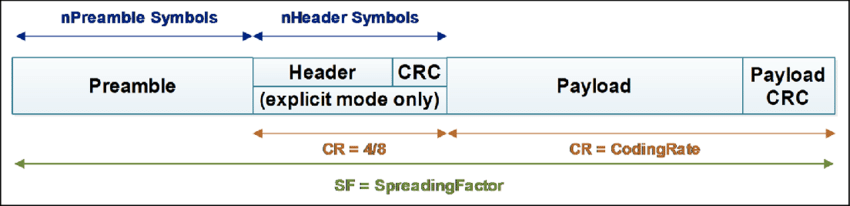
\includegraphics[scale=0.4]{images/lorapacket.png}
\caption{Structure d'un paquet Lora\cite{lorapacket}}\label{term6}
\end{figure}


La figure \ref{term6} montre la structure d'un paquet Lora. Un paquet LoRa contient 3 parties différentes \cite{loraphy} :

\vspace{0.1cm}

\begin{itemize}
\item Le \textit{preamble}. La première partie du paquet, composée d'un nombre variable d'upchirps. La valeur par défaut est fixée à 8 upchirps minimum. L'émetteur radio ajoute à cela un peu plus de 4 symboles (4.25), qui contiennet l'identificateur réseau ainsi que deux downchirps de synchronisation de fréquence. Ceci fixe le préambule à 12 symboles.
\item Le \textit{header} du paquet. Les informations sur la taille du paquet, le code rate, la présence d'un CRC (\textit{cyclique redundancy check}) et la checksum sont incluses dans l'en-tête.
\item Le \textit{payload}. La dernière partie du paquet qui contient les données à transmettre. La taille maximale du payload est de 255 octets. En plus des données, le payload peut également contenir un CRC pour la détection d'erreurs. La longueur du CRC est généralement de 16 bits.
\end{itemize}


\subsection{LoRaWAN}\label{lorawan}

LoRaWAN est un protocol de type \textit{Low Power Wide Area Network (LPWAN)} désigné pour la communication longue portée. Ce protocole opère avec la technologie LoRa et lui fournit une infrastructure capable de maintenir une communication à longue portée et à faible cout dans l'IoT.

\subsubsection{Aspets généraux de la technologie}

LoraWan bénéficie donc d'une faible puissance de consommation et d'une portée accrue. Elle est également efficace dans différents environements. Le signal est capable de pénétrer diverses terrains et structures.
Le déploiment d'une infrastructure LoRa ne nécessite pas de license, et son réseau peut être public ou privé. Les caractéristiques générales de LoraWan sont disponibles sur le site \href{https://www.thethingsnetwork.org/docs/lorawan/}{The Thing Network}.

\vspace{0.1cm}

Le coeur de LoRaWAN réside sur la gestion de l'énergie, permettant aux appareils de fonctionner avec une consommation d'énergie minimale, prolongeant leur durée de vie tout en garantissant une fonctionnalité à long terme. A cette caractéristique de faible consommation d'énergie s'ajoute ses capacités en termes de portée, capable de pénéter diverses environements. Cela rend la technologie efficace aussi bien milieu rurale qu'urbain. LoRaWAN opère sur une bande de fréquence qui ne nécessite pas de license d'émition, par exemple sur la bande ISM pour \textit{Industrial, Scientific, and Medical}. Les bandes ISM, (868 MHz en Europe ou 915 MHz aux USA) sont disponibles pour l'utilisation de différentes technologies, incluant LoraWAN.

\vspace{0.1cm}

LoRaWAN possède des capacités de géolocalisation, permettant au réseau de détecter et de localiser précisément les appareils au sein de son domaine. LoraWAn utilise différentes méthodes pour localiser ses appareils comme \textit{Received signal strengh indication (RSSI)}, \textit{Time difference on Arrival (TDOA)}, une triangulation ou alors une combinaison de plusieurs des méthodes. Certaines de ses méthodes seront détaillées dans la section \ref{identification}

\vspace{0.1cm}

LoRaWAN utilise des protocoles de sécurité \textit{end-to-end}, aussi bien dans un réseau public intégré que dans un réseau privé.L'architecture LoraWan (décrite en détails dans la section \ref{topolora}) contient plusieurs couches de sécurité. Au niveau des \textit{end devices}, une routine d'identification est imposée avant l'accès au réseau. seul les appareils de confiance son donc autorisé à communiquer. Ensuite, une fois la communication commencée, les données sont chiffrées avant d'être transmise dans le réseau. Le framework sécuritaire de Lora ne se limite pas à l'autentification et au chiffrage. LoraWan gère également les mise à jour en continue par les airs, ainsi qu'une supervision continue sur d'éventuelles intrusions.

\vspace{0.1cm}

Avec toutes ces caractéristiques, LoraWan s'est développé dans de nombreux domaines aussi bien environementaux qu'industriels. Les principales utilisations de LoraWan actuelles sont les suivantes (toutes les applications \href{https://www.semtech.com/lora/lora-applications}{ici}):

\vspace{0.1cm}

\begin{itemize}

\item la surveillance environementale en général \cite{lorauc1}. Lorawan peut être déployé pour surveiller des niveaux de températures, d'humidité, de bruits ou encore d'autres paramètres dans n'importe quel milieu. Une compagnie Hollandaise, \href{https://www.sensoterra.com/technology/global-lorawan-networks/}{Sensoterra}, utilise notamment LoraWan pour surveiller la qualité des sols.
\item Les \textit{smart cities} \cite{lorauc2}. LoraWan est actif sur différents aspects comme la gestion intelligent de l'éclairage, la gestion des déchets, la surveillance, etc.
\item l'embarqué industriel \cite{lorauc3}. La maintenance et la surveillance de matériel et de l'équipement peut être gérée par Lorawan. \href{https://consulting.tatasteel.com/our_expertise/plant-infrastructure-and-logistics/}{TataSteel}, une compagnie indienne, utilise LoraWan pour ces équipements industriels.
\item la prévention de catastrophe naturelle. Que ce soit en prévision\cite{lorauc41} ou après\cite{lorauc43} d'éventuelles catastrophes naturelles, la longue portée et la surveillance en temps réel sont des atoux cruciaux pour ce genre d'évènement.
\end{itemize}

\vspace{0.1cm}

Cependant, toutes ses caractéristiques entrainent un certain nombre de limitations. La restriction de la fréquence en fonction de la région peut rendre le déploiment d'une même infrastructure à différent endroit dans le monde plus difficile. Cela peut aussi entrainer des problèmes de compatibilité entre régions, notament pour des chaines logistique ou d'approvisionement qui en traverse plusieurs.

\vspace{0.1cm}

Une faible consommation de puissance avec une grande portée a un impact sur la taille et la vitesse de l'information. La taille du payload d'un message est limitée entre 51 et 241 octets. La vitesse de transmission est également peu élevée, atteignant un maximum de 5.5kbps sur une largeur de bande de 125kHz.

\vspace{0.1cm}

La communication au sein d'un réseau LoraWan se fait en grande partie de manière asynchrone. La synchronisation dépend de la classe de l'appareils, qui est détaillé dans la section \ref{topolora}. C'est un avantage pour maintenir une grande autonomie de batterie pour les appareils. LoraWan possède un système pour limiter les colisions entre messages si plusieurs appareils communiquent simultanénent. Ce système est basé sur une combinaison entre \textit{Listen before talk (LBT)} et des delais aléatoires\cite{loracolision}. Il est néamoins possible que dans un environement très dense des collisions puissent encore se produire. La comunications asynchrone et le système d'évitement de collision entraine une augmentation du temps entre les envois et la réception de message.

\subsubsection{Topologie de Lorawan}\label{topolora}

\begin{figure}[h]
\centering

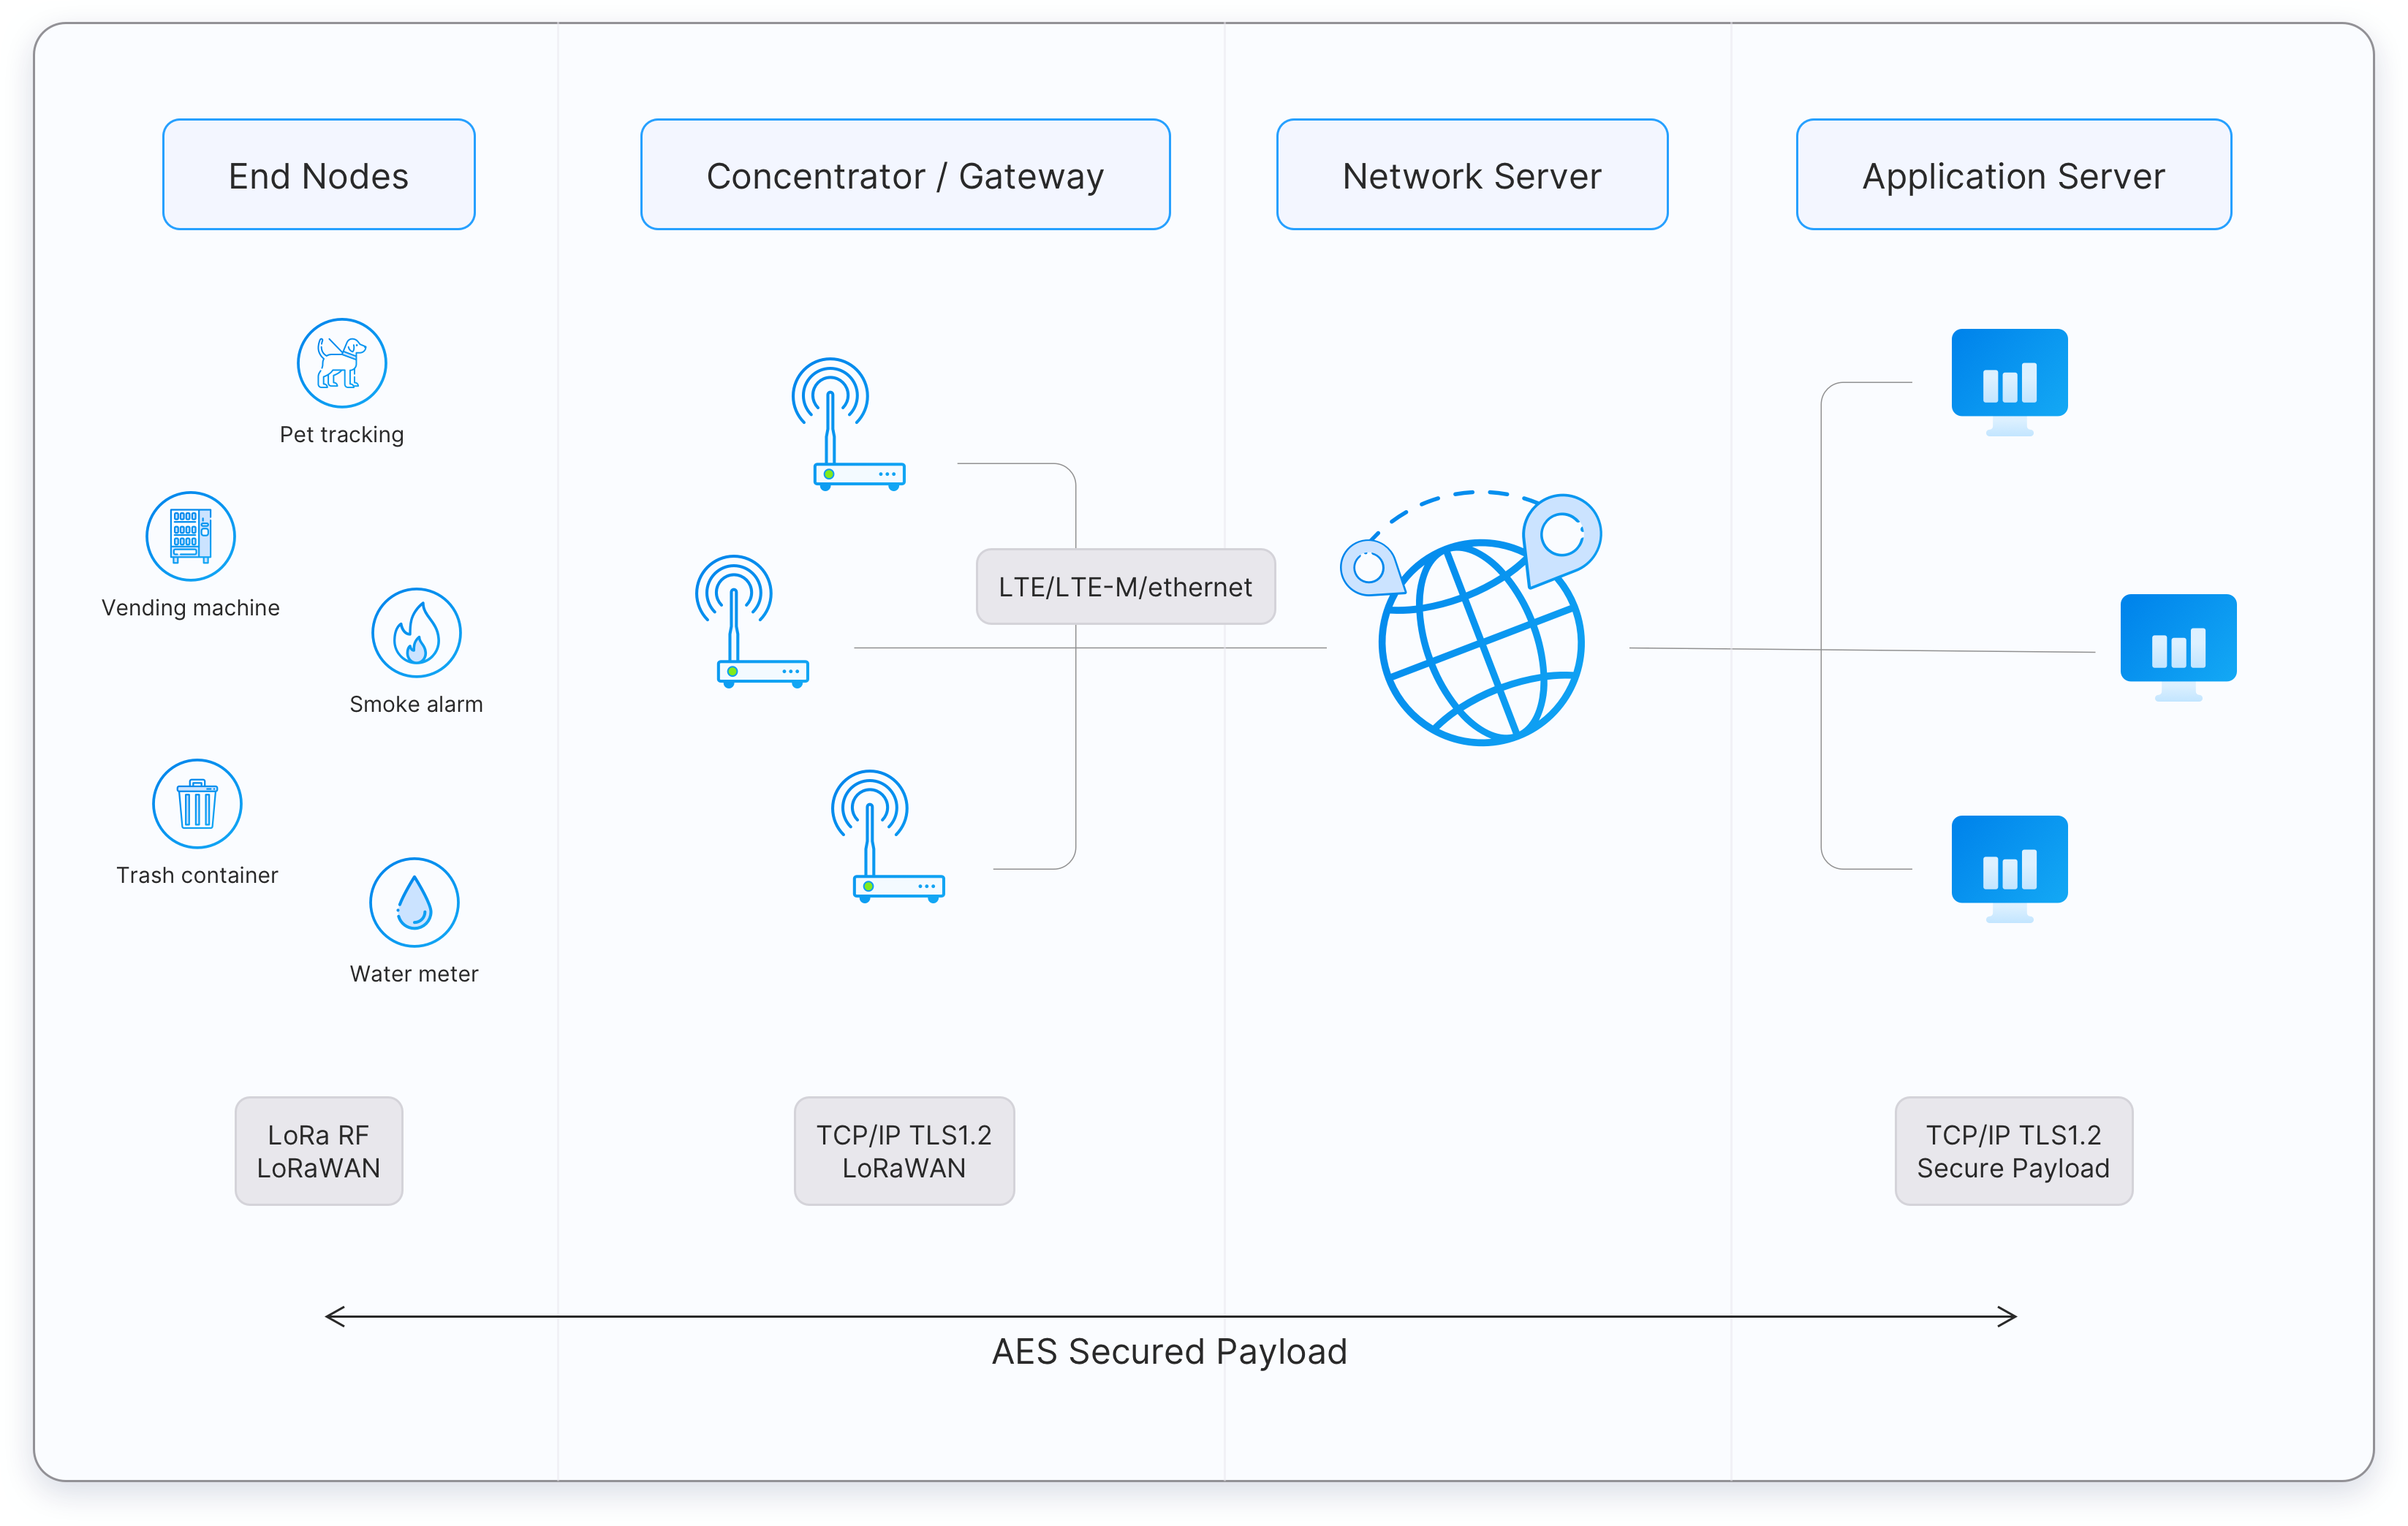
\includegraphics[scale=0.1]{images/architecture.png}
\caption{Topologie de l'infrastructure LoraWan (source : \href{https://www.thethingsnetwork.org/docs/lorawan/architecture/}{The Thing Newtork})}\label{term7}
\end{figure}

La figure \ref{term7} montre les 4 types d'appareils qui composent la topologie d'un infrastrucure LoraWan.
Les end devices sont les noeuds qui collectent les informations à envoyer à travers le réseau. Ils sont catégorisés en trois sous classes : A, B et C. Les apareils de classe A sont les plus économes en énergie. Ils ont été créés pour conserver leur énergie et communiquent exclusivement en comunication asynchrone. Les appareils de classe A écoutent les messages provenant des serveurs uniquement après avoir eux-même transmis un message. la classe A regroupe les appareils les moins énergivores. Les appareils de classe B sont assez similaires à ceux de classe A, mais sont occasionellement synchronisés avec les serveurs du réseau. Ils possèdent des capacités supérieurs de reception leur permettant de se synchroniser avec le scheduler des serveurs, ce qui augmente considérablement l'efficacité du temps de réponses dans le réseau. Finalement, les appareils de classe C sont en écoute permanente de messages provenant des serveurs. Ils sont les plus réactifs mais également les plus énergivores. Les end devices sont donc classés selon deux paramètres : leur réactivité et leur consomation d'énergie. En fonction de leur classe, ils ont également la possibilité de recevoir des messages server après avoir transmis de l'information. L'envoie d'un message d'un end devices vers les serveurs est appelé \textit{uplink message} et l'envoie d'un message depuis les serveur vers les end devices est appelée \textit{downlink message}.

\vspace{0.1cm}

Les gateways jouent le role d'intermédiaire entre les end devices et le serveur réseau. Ils recoivent les transmissions depuis les end devices dans leur zone de couverture
et forward les messages vers le serveur réseau. Les gateways peuvent écouter plusieurs fréquence simultanénent (\textit{multichanneling}) là où les end devices n'écoutent qu'une seule fréquence. Les gateway gèrent la communication radio avec les end devices en utilisation la modulation de LoRa.

\vspace{0.1cm}

Le serveur réseau est la composante centrale de l'infrastructure. Il gère tout le réseau, que ce soit les données reçues des gateays, l'identification et l'activation des end devices dans le réseau, le routing ou encore l'adapation du data rate. Le serveur réseau supervise également l'aspect sécurité au sein du réseau en gèrant les clés de chiffrage et les protocoles de sécurité.

\vspace{0.1cm}

Le serveur application de LoraWan reçoit les données forwardées depuis le serveur réseau. C'est l'interface entre le réseau de LoraWan et les différents services ou applications d'utilisaturs finaux. Les utilisateurs intéragissent avec le serveur d'application pour n'importe quelle action a effectuer sur le réseau ou pour la récupération de données du réseau. Les données reçues par le serveur réseau sont traduites par le server d'application avant d'être interprétée par l'utilisateur final.

\subsubsection{Sécurité}

La sécurité dans l'architecture LoraWan se concentre sur trois axe principaux :

\begin{itemize}
\item l'authentification : qui communique avec qui.
\item L'intégrité : les données ne sont pas altérées entre l'émetteur et le recepteur.
\item La confidentialité : les données ne sont visible par personne au sein du réseau hormi l'émetteur et le récepteur. 
\end{itemize}

\vspace{0.1cm}

La sécurité repose sur le chiffrage des données. Les données sont chiffrées en utilisant l'algorithme de cryptographie AES (\textit{Advanced Encryption Standard}). La taille des clés est de 128 bits. Ce choix est motivé par un équilibre entre une sécurité suffisante et une consommation réduite des ressources\cite{loraes}.

\vspace{0.1cm}

Il y a deux types de clés utilisées dans LoraWan. La \textit{root key} est la clé partagée entre un end device et le serveur réseau. Cette clé est utilisée pour l'authentification initiale et l'établissement d'une communication entre deux éléments du réseau. Cette clé n'est jamais transmise par les air, elle est stockée dans un \textit{join server}. Un join server est un server dédié au contenu sensible à l'activation du matériel dans un réseau LoRaWAN. Il autentifie le réseau et les application du servers. Il gère les root keys. il génère également le second type de clés de LoraWan, les \textit{session keys}.

Les session keys sont des clés générées dynamiquement par le join server et utilisées durant l'échange de données pendant une session. Il y a deux session keys différente, la \textit{AppSKEY} pour le chiffrage des payloads d'application, et la \textit{nwkSKEY} pour les fonctionalités du réseau (le chifrage à la couche MAC, les vérification d'integrité, etc).

\subsubsection{Session}

L'établissement d'une session entre un end devices et le réseau LoraWan peut se faire de deux façons différentes.

La première méthode est une méthode dynamique appelée \textit{Over the Air Activation(  OTAA)} et se déroule de la façon suivante: 
\begin{itemize}
\item Le device possède initialement deux indentificateurs, un DevEUI et un appEUI.
\item La requête pour rejoindre le réseau est initiée par le end device. Il en envoir un message \textit{join request} au serveur réseau. La join request contient ses identificateurs, ainsi qu'un nombre aléatoire généré par le device.
\item Le serveur réseau accepte (ou décline) la requête et vérifie les identifiateurs du device dans ses enregistrements. 
\item Si la requête est acceptée, le server génère ensuite un nombre aléatoire appelé \textit{DevNonce} et renvoie un message \textit{join accept} contenant le DevNonce, l'adresse du device ainsi que les clés (NwkSKey et appSKey) de session.
\item le end device reçoit le message join accept. Il extrait les clés envoyées et calcule ses propres clés de session avec ses paramètres (les clés envoyé par le join server ainsi que le devNonce).
\item le device fait maintenant parti du réseau. Chaque message que le device va envoyer au serveur sera chiffré avec ses clés.
\end{itemize}
        
\vspace{0.1cm}
        
La seconde méthode est hardcodée et permet à un end device de rejoindre directement le réseau sans passer par l'indentification. cette méthode est appelée \textit{activation by personalisation (ABP)}. Voici la procédure de la session :
\begin{itemize}
\item Le device possède à l'avance son adresse ainsi que ses clés de session.
\item Le device est déploiyé au préalable dans la zone de couverture du réseau LoraWan.
\item Sans devoir itinialiser de procedure \textit{join request}, le end device transmet directement ses données au serveur en utilisant ses clés préconfigurées. L'échange de clés avec le serveur n'a pas lieu.
\end{itemize}

Cette seconde procèdure a comme avantage d'être plus rapide à exécuter car toute la partie d'initialisation est passée. Le processus d'initialisation peut être contraignant en ressource ce qui rend la méthode ABP moins énergivore. Cependant l'utilisation de clés hardcodées directement dans les devices est une pratique moins sécuritaire. Comme pour la taille de clés, il y a un équilibre entre consommation d'énergie et sécurité.
